\chapter{Lab Techniques III: Research Practice}\label{ch:b3:lab-techniques-3}

A bottle of butyllithium solution catches fire if a drop meets the air; a
\omterm{def:b3:lab-techniques-3:schlenk}{glovebox} keeps oxygen and water below a few parts per million so that such
compounds can be weighed like table salt. Research chemistry often begins by
keeping the atmosphere out, and ends with a claim that others must be able to
check: a new compound, its structure and purity proved by several independent
methods, its data recorded and published so that the work can be repeated. This
last chapter gathers the practice of research: handling air-sensitive
substances, characterising a new compound, judging a result statistically,
keeping a notebook and reading the literature, and assessing the risks of a
procedure no one has run before.

\begin{recall}
The Year 1 volume treated hazards, risks, pictograms, H and P statements, safety
data sheets and measurement uncertainty with its type A and B evaluations; the
Year 2 volume inert atmospheres, work-up, drying agents, flash chromatography,
mass spectrometry (HRMS, monoisotopic mass), $^{13}$C NMR, confidence intervals,
Student's coefficient, calibration, precision, trueness, bias, repeatability,
method validation, the adiabatic temperature rise and thermal runaway.
\Cref{ch:b3:advanced-nmr}, \cref{ch:b3:x-ray-diffraction} and
\cref{ch:b3:electrode-kinetics} supplied the structural and electrochemical
methods.
\end{recall}

\begin{omfigure}
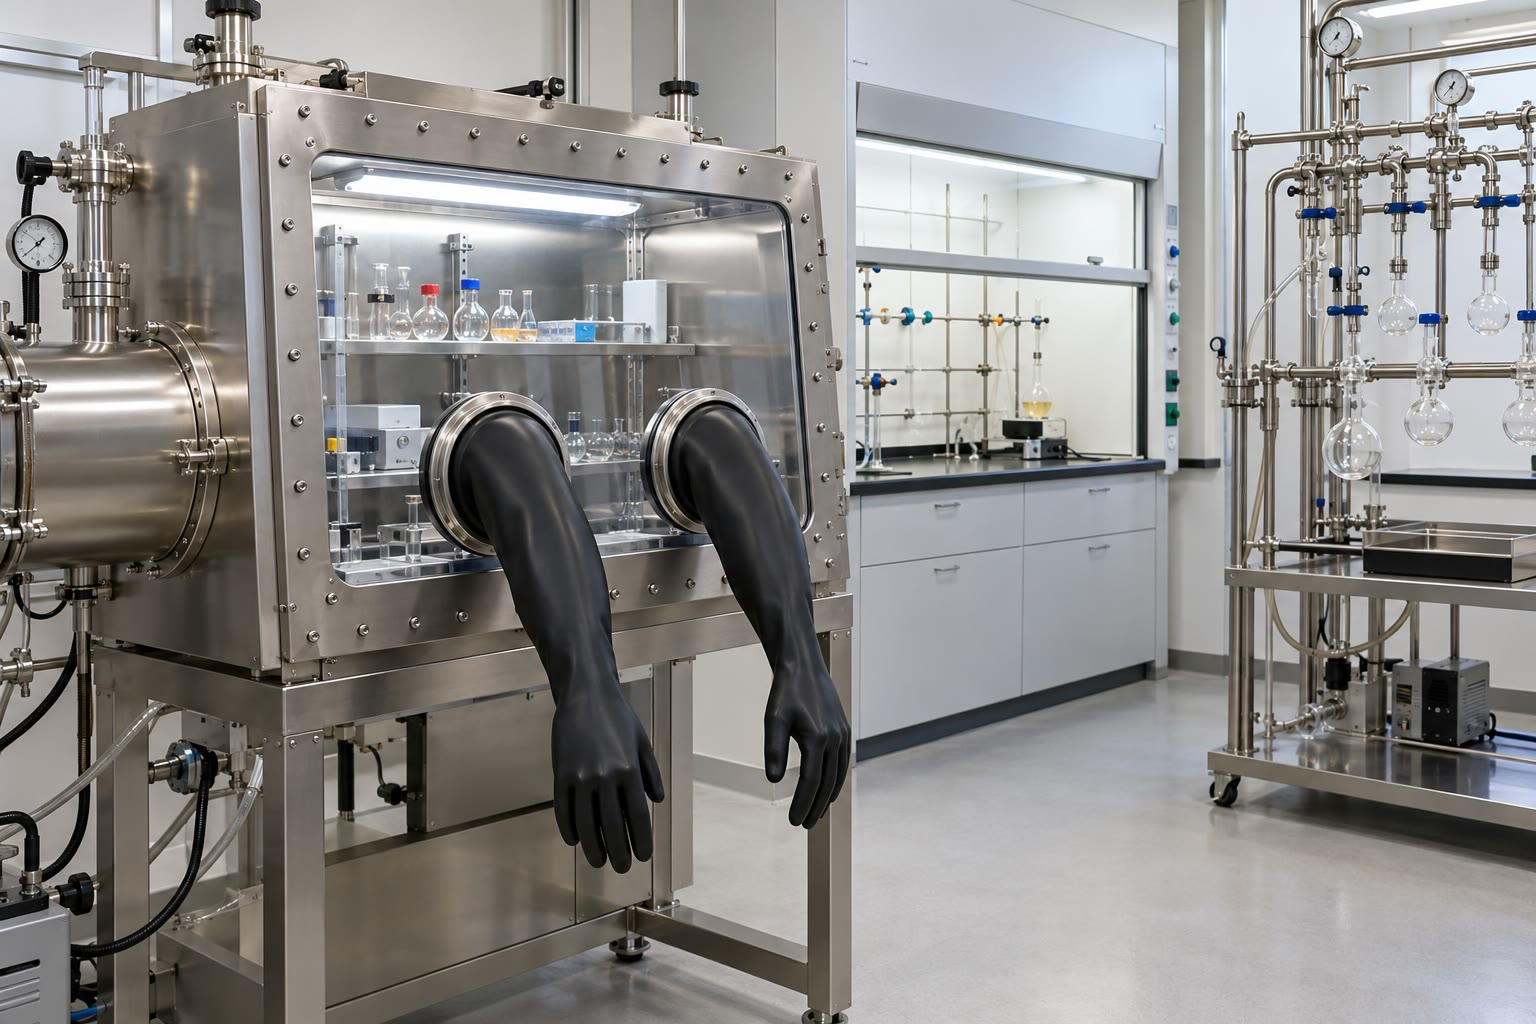
\includegraphics[width=0.58\linewidth]{images/book4/ai/b3-33-glovebox.jpg}

{\small A research laboratory with a \omterm{def:b3:lab-techniques-3:schlenk}{glovebox}: the stainless-steel box, filled
with dry nitrogen or argon, is entered through the gloves; the cylinder on the
left is the antechamber for bringing items in and out.}
\end{omfigure}

\section{Working without air}

\begin{definition}[Air-sensitive compounds]\label{def:b3:lab-techniques-3:air-sensitive}
An \emph{air-sensitive compound}\index{air-sensitive compound} reacts with
dioxygen or water of the air, decomposing or losing its activity. A
\emph{pyrophoric substance}\index{pyrophoric substance} ignites spontaneously in
air.
\end{definition}

\begin{definition}[Schlenk line and glovebox]\label{def:b3:lab-techniques-3:schlenk}
A \emph{Schlenk line}\index{Schlenk line} is a double glass manifold, one tube
connected to a vacuum pump through a cold trap, the other to a supply of dry inert
gas vented through an oil bubbler, with taps that connect each outlet to
either. A \emph{Schlenk flask}\index{Schlenk flask} has a side arm with a tap
for connection to the line. A \emph{glovebox}\index{glovebox} is a sealed box
filled with inert gas, continuously purified, in which work is done through
gloves.
\end{definition}

\begin{omfigure}
\begin{tikzpicture}[font=\scriptsize, >=Stealth]
  % manifolds
  \draw[om glass, line width=1.1pt] (0,3.0) -- (8.0,3.0);
  \draw[om glass, line width=1.1pt] (0,2.5) -- (8.0,2.5);
  \node[anchor=east] at (-1.0,3.0) {inert gas};
  \node[anchor=east] at (0,2.5) {vacuum};
  % taps
  \foreach \x in {2.0,4.0,6.0} {
    \draw[om glass] (\x,3.0) -- (\x,2.5);
    \draw[fill=white] (\x,2.75) circle (0.12);
    \draw (\x-0.1,2.75) -- (\x+0.1,2.75);
    \draw[om glass] (\x,2.5) -- (\x,2.0);
  }
  % flask on the middle tap
  \draw[thick, black!60] (4.0,2.0) -- (4.0,1.6) -- (4.6,1.6);
  \pic[scale=0.5, transform shape] at (5.0,-0.2) {rbflask={0.3}{omDef!20}};
  \draw[om glass] (4.6,1.6) -- (4.9,1.25);
  \node[anchor=west] at (5.4,0.4) {Schlenk flask};
  % bubbler at the gas end
  \pic[scale=0.55, transform shape] at (8.9,1.5) {bubbler};
  \draw[om glass] (8.0,3.0) -- (8.6,3.0) -- (8.6,2.9);
  \node[anchor=west] at (9.4,2.2) {oil bubbler};
  % trap and pump at the vacuum end
  \draw[om glass] (0.4,2.5) -- (0.4,1.6);
  \draw[om glass, fill=omDef!8] (0.15,1.6) rectangle (0.65,0.4);
  \fill[omDef!25] (0.0,0.2) rectangle (0.8,1.2);
  \node[anchor=north] at (0.4,0.2) {cold trap};
  \draw[om glass] (0.65,0.9) -- (1.6,0.9);
  \draw[fill=black!15] (1.6,0.6) rectangle (2.6,1.2);
  \node at (2.1,0.9) {pump};
  \draw[->, thick] (-0.9,3.0) -- (0,3.0);
\end{tikzpicture}

{\small A \omterm{def:b3:lab-techniques-3:schlenk}{Schlenk line}, schematic: a gas manifold and a vacuum manifold joined by
taps; each tap connects its flask either to vacuum or to inert gas. Solvent vapour
pumped off condenses in the cold trap before it reaches the pump; the gas leaves
through an oil bubbler, which keeps air from flowing back.}
\end{omfigure}

\begin{proposition}[Evacuate--refill cycles]\label{prop:b3:lab-techniques-3:purge-cycles}
If a flask filled with air at pressure $p_0$ is evacuated to $p_{\min}$ and refilled with
pure inert gas, $n$ times, the fraction of the original air left is $(p_{\min}/p_0)^n$.
\end{proposition}

\begin{proof}
Evacuating to $p_{\min}$ leaves a fraction $p_{\min}/p_0$ of the gas, of the same composition; the
refill with pure inert gas restores $p_0$ without adding air. Each cycle multiplies the
air fraction by $p_{\min}/p_0$; after $n$ cycles, $(p_{\min}/p_0)^n$.
\end{proof}

Three cycles to \qty{0.1}{mbar} leave on paper $10^{-12}$ of the air; in practice leaks, gas
adsorbed on the glass and outgassing of grease and septa set the limit, which is
why glassware is dried in an oven and assembled hot.

\begin{definition}[Cannula transfer]\label{def:b3:lab-techniques-3:cannula}
A \emph{cannula transfer}\index{cannula transfer} moves an air-sensitive liquid
from one sealed vessel to another through a long double-tipped needle, driven
by a small overpressure of inert gas in the first vessel.
\end{definition}

\begin{omfigure}
\begin{tikzpicture}[font=\scriptsize, >=Stealth]
  \pic at (0,0) {rbflask={0.35}{omThm!25}};
  \pic at (4.2,0) {rbflask={0.1}{omDef!15}};
  \pic at (0,3.0) {septum};
  \pic at (4.2,3.0) {septum};
  \draw[black!70, line width=0.9pt] (0.05,0.25) -- (0.05,3.5) to[out=90, in=90] (4.15,3.5) -- (4.15,1.6);
  \draw[->, thick, omThm] (1.3,3.95) -- (2.9,3.95) node[midway, above] {liquid};
  \draw[->, thick] (-1.3,3.4) -- (-0.15,3.2) node[pos=0, left] {inert gas in (slight overpressure)};
  \draw[->, thick] (4.35,3.2) -- (5.4,3.6) node[right] {vent to bubbler};
  \node[anchor=north] at (0,-0.1) {source};
  \node[anchor=north] at (4.2,-0.1) {receiver};
\end{tikzpicture}

{\small A \omterm{def:b3:lab-techniques-3:cannula}{cannula transfer}: the cannula's lower tip dips into the liquid of the
source flask; inert gas let into the source pushes the liquid through the
cannula into the receiver, which is vented through a needle to the bubbler.}
\end{omfigure}

\begin{method}[A cannula transfer]\label{met:b3:lab-techniques-3:cannula}
\begin{enumerate}
  \item Put both flasks, sealed with septa, under inert gas on the \omterm{def:b3:lab-techniques-3:schlenk}{Schlenk line}.
  \item Purge the cannula with gas: insert one end into the source above the liquid
        until gas flows out of the other end, then insert that end into the receiver.
  \item Vent the receiver with a needle; push the cannula's source end below the
        liquid surface: the overpressure drives the liquid across.
  \item To stop, lift the tip above the liquid; withdraw the cannula from the receiver
        first, and rinse it at once with a dry solvent, then with water, in the hood.
\end{enumerate}
\end{method}

\begin{definition}[Freeze--pump--thaw degassing]\label{def:b3:lab-techniques-3:degassing}
\emph{Freeze--pump--thaw degassing}\index{freeze--pump--thaw degassing} removes
dissolved gases from a liquid by freezing it in liquid nitrogen, evacuating the
space above it, closing the tap and letting it thaw, so that dissolved gas escapes
into the vacuum; the cycle is repeated three times.
\end{definition}

Dry solvents now come from columns of activated alumina under inert gas
rather than from stills over sodium. Organolithium solutions lose strength with
time and are titrated before use, for instance against a weighed amount of
diphenylacetic acid in dry THF: the first equivalent deprotonates the acid, the
first drop in excess gives the yellow dianion.

\begin{proposition}[Titre of an organolithium]\label{prop:b3:lab-techniques-3:titre}
If a mass $m$ of diphenylacetic acid (molar mass $M$) needs a volume $V$ of an
organolithium solution to reach the colour change, the concentration is $c = m/(MV)$.
\end{proposition}

\begin{proof}
Up to the end point each organolithium removes one proton from the acid; the
colour appears when the acid is used up. The amounts are equal: $cV = m/M$.
\end{proof}

\begin{inthelab}[The glovebox antechamber]
Items go into a \omterm{def:b3:lab-techniques-3:schlenk}{glovebox} through its antechamber: they are placed inside, the
outer door is closed, and the chamber is evacuated and refilled with the box's
gas three times, with a long final evacuation for porous items, which hold air;
only then is the inner door opened from inside the box with the gloves. Solvents
and open containers of volatile liquids are never pumped in the antechamber, and
nothing that would poison the purifier (thiols, halogenated solvents) is opened
inside without permission.
\end{inthelab}

\begin{omfigure}
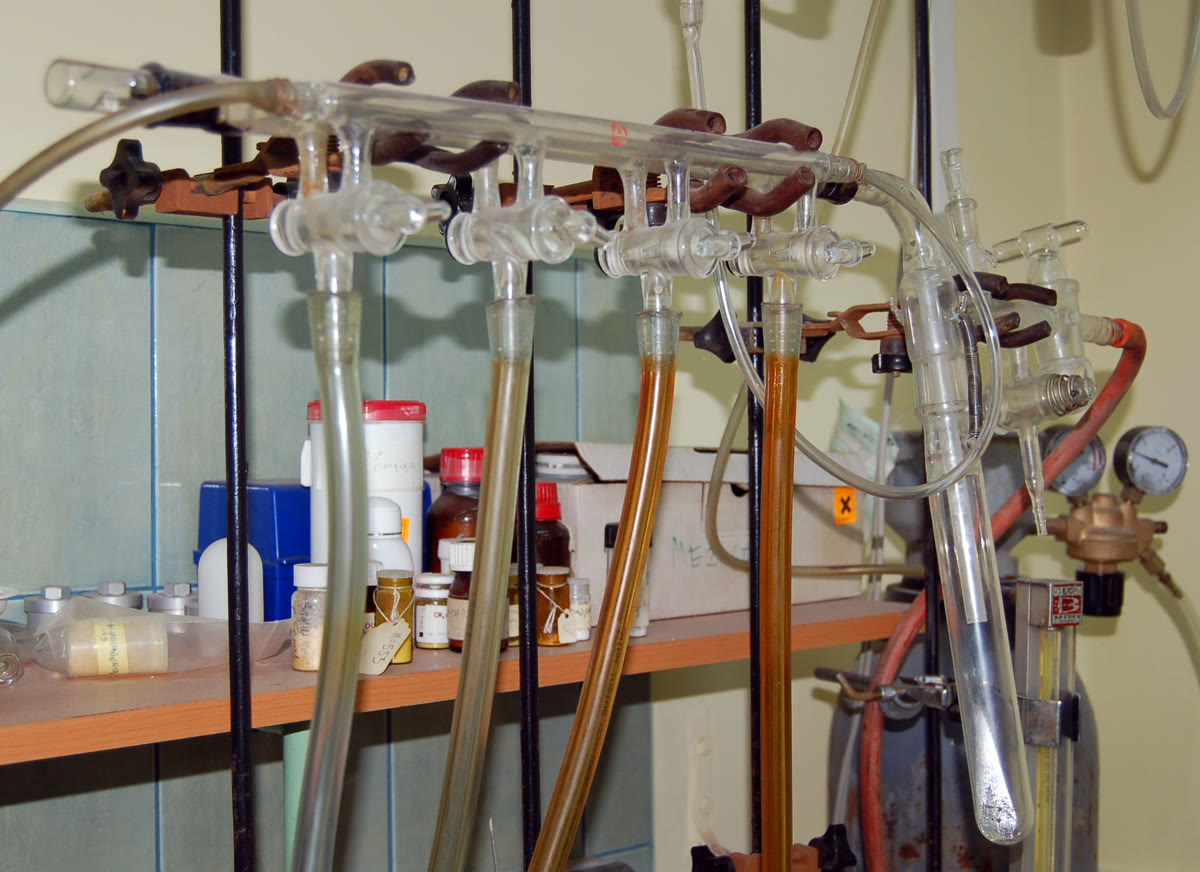
\includegraphics[width=0.46\linewidth]{images/book4/schlenk-line.jpg}

{\small A \omterm{def:b3:lab-techniques-3:schlenk}{Schlenk line} in use: the glass manifold with its taps, tubing to the
flasks, and the gas regulator. Photograph: Polimerek, CC BY-SA 3.0.}
\end{omfigure}

\section{Characterising a new compound}

\begin{method}[Characterising a new compound]\label{met:b3:lab-techniques-3:characterise}
\begin{enumerate}
  \item Purity: one spot in TLC in two eluents, one peak in HPLC or GC, a sharp
        melting point; \omterm{def:b3:lab-techniques-3:qnmr}{quantitative NMR} if a mass purity is needed.
  \item Formula: HRMS within a few ppm of the calculated mass, and the isotope
        pattern; or \omterm{def:b3:lab-techniques-3:elemental}{elemental analysis}.
  \item Structure: $^1$H and $^{13}$C NMR with 2D experiments for the connections
        (\cref{ch:b3:advanced-nmr}), IR for the functional groups; a single-crystal
        X-ray structure when crystals grow (\cref{ch:b3:x-ray-diffraction}).
  \item Stereochemistry: NOE, coupling constants, optical rotation, ee by chiral
        chromatography.
  \item Report every datum with its conditions, and the spectra in the \omterm{def:b3:lab-techniques-3:literature}{supporting
        information}.
\end{enumerate}
\end{method}

\begin{omfigure}
\begin{tikzpicture}[font=\scriptsize, >=Stealth,
  box/.style={draw, rounded corners, align=center, fill=omDef!8, inner sep=3pt, minimum height=8mm}]
  \node[box] (a) at (0,0) {new compound\\ isolated};
  \node[box] (b) at (2.85,0) {pure?\\ TLC, HPLC, m.p.};
  \node[box] (c) at (5.85,0) {formula\\ HRMS, CHN};
  \node[box] (d) at (8.75,0) {structure\\ NMR (1D, 2D), IR};
  \node[box] (e) at (8.75,-1.6) {X-ray if crystals,\\ stereochemistry};
  \node[box, fill=omMeth!12] (f) at (5.85,-1.6) {consistent?\\ report with\\ raw data};
  \node[box, fill=omThm!10] (g) at (2.85,-1.6) {purify again\\ (chromatography,\\ crystallisation)};
  \draw[->, thick] (a) -- (b); \draw[->, thick] (b) -- node[above, inner sep=1pt] {yes} (c);
  \draw[->, thick] (c) -- (d); \draw[->, thick] (d) -- (e); \draw[->, thick] (e) -- (f);
  \draw[->, thick] (b) -- node[left] {no} (g); \draw[->, thick] (g.north west) to[bend left=30] (a.south);
\end{tikzpicture}

{\small The characterisation workflow of a new compound: purity first, then the
formula, then the structure; every claim rests on at least two independent
methods, and the \omterm{def:b3:lab-techniques-3:notebook}{raw data} go with the report.}
\end{omfigure}

\begin{definition}[Elemental analysis]\label{def:b3:lab-techniques-3:elemental}
\emph{Elemental analysis}\index{elemental analysis} (combustion analysis)
determines the mass percentages of carbon, hydrogen, nitrogen and sulfur in a
sample by burning it in oxygen and measuring the carbon dioxide, water,
dinitrogen and sulfur dioxide formed.
\end{definition}

\begin{proposition}[Mass percentages from a formula]\label{prop:b3:lab-techniques-3:mass-fractions}
For a formula $\mathrm{C}_a\mathrm{H}_b\mathrm{N}_c\dots$ of molar mass $M$, the mass percentage of carbon is $100\,aA_r(\mathrm C)/M$, and likewise
for the other elements.
\end{proposition}

\begin{proof}
One mole of compound, of mass $M$, contains $a$ moles of carbon atoms, of mass $aA_r(\mathrm C)$;
the ratio, times 100, is the mass percentage.
\end{proof}

% ledger: ea:tolerance, hrms:tolerance
Most chemistry journals ask for found C, H and N values within 0.4 percentage
points of the calculated ones, or for an HRMS measurement within a few ppm (5 ppm
for some), as evidence of composition. A large interlaboratory study found that
even pure samples miss the 0.4 criterion surprisingly often, a reminder that a
criterion is not a law of nature.

\begin{proposition}[HRMS error]\label{prop:b3:lab-techniques-3:ppm-error}
The error of a measured mass $m_{\mathrm{meas}}$ against the calculated $m_{\mathrm{calc}}$ is
$10^6(m_{\mathrm{meas}} - m_{\mathrm{calc}})/m_{\mathrm{calc}}$ ppm; for an ion, $m_{\mathrm{calc}}$ is computed from monoisotopic masses minus (or plus) the
mass of the electrons removed (or added).
\end{proposition}

\begin{proof}[By definition]
The ppm error is the relative difference expressed in parts per million; the
ion's mass differs from the neutral formula's by the electrons, \qty{5.486e-4}{u} each, a
few ppm at masses of a few hundred.
\end{proof}

\begin{definition}[Quantitative NMR]\label{def:b3:lab-techniques-3:qnmr}
\emph{Quantitative NMR}\index{quantitative NMR} (qNMR) determines amounts or
purities from signal integrals, which are proportional to the number of nuclei
when the spectrum is recorded with full relaxation between pulses, against an
internal standard of known purity weighed with the sample.
\end{definition}

\begin{proposition}[qNMR purity]\label{prop:b3:lab-techniques-3:qnmr}
For a sample of mass $m_x$ weighed with a standard of mass $m_s$ and purity $P_s$, with signals
of integrals $I_x$ and $I_s$ from $N_x$ and $N_s$ protons,
\[
  P_x = \frac{I_x}{I_s}\,\frac{N_s}{N_x}\,\frac{M_x}{M_s}\,\frac{m_s}{m_x}\,P_s.
\]
\end{proposition}

\begin{proof}
The integrals are proportional to the numbers of protons: $I_x/I_s = (N_xn_x)/(N_sn_s)$. With
$n_x = P_xm_x/M_x$ and $n_s = P_sm_s/M_s$, solving for $P_x$ gives the formula.
\end{proof}

\begin{omfigure}
\begin{tikzpicture}
\begin{axis}[width=0.8\linewidth, height=5.0cm, x dir=reverse, xmin=3.0, xmax=7.0, ymin=-0.05, ymax=1.15, clip=false,
  axis x line=bottom, axis y line=none, xlabel={$\delta$ / ppm}, tick label style={font=\scriptsize}, label style={font=\small}]
\addplot[color=omDef, thick] table[x=ppm, y=y] {figdata/out/bachelor-3-qnmr.dat};
\node[font=\scriptsize, anchor=south] at (axis cs:6.09,0.33) {standard, ArH (3 H)};
\node[font=\scriptsize, anchor=east] at (axis cs:4.20,0.98) {ferrocene (10 H)};
\node[font=\scriptsize, anchor=west, align=left] at (axis cs:3.72,0.70) {standard,\\ $\ce{OCH3}$ (9 H)};
\end{axis}
\end{tikzpicture}

{\small Synthetic proton spectrum of a ferrocene sample weighed with
1,3,5-trimethoxybenzene as internal standard (model: 20.0 mg of sample of 98.0\,\%
purity, 15.0 mg of standard). The integrals are proportional to the number of
protons times the amount of each compound; the ratio of the ferrocene singlet to
the standard's aromatic singlet gives the purity.}
\end{omfigure}

\section{Statistics of a research result}

\begin{definition}[Significance tests]\label{def:b3:lab-techniques-3:tests}
A \emph{significance test}\index{significance test} decides whether data are
compatible with a \emph{null hypothesis}\index{null hypothesis}, usually that
there is no difference or no effect, at a chosen level of risk of rejecting it
wrongly (often 5\,\%).
\end{definition}

\begin{theorem}[Two-sample $t$ test]\label{thm:b3:lab-techniques-3:t-test}
For two sets of $n_1$ and $n_2$ independent measurements drawn from normal
distributions of equal standard deviation, with means $\bar x_1$, $\bar x_2$ and pooled
standard deviation $s_p$, the statistic $t = (\bar x_1 - \bar x_2)/(s_p\sqrt{1/n_1 + 1/n_2})$ follows Student's law with
$n_1 + n_2 - 2$ degrees of freedom when the two true means are equal. \admitted
\end{theorem}

\begin{proposition}[$F$ test]\label{prop:b3:lab-techniques-3:f-test}
Under the same assumptions, the ratio $F = s_1^2/s_2^2$ of two sample variances follows
Fisher's law with $(n_1 - 1, n_2 - 1)$ degrees of freedom when the true variances are equal.
\admitted
\end{proposition}

\begin{method}[Is a new yield better?]\label{met:b3:lab-techniques-3:compare-means}
\begin{enumerate}
  \item Repeat both procedures several times under the same conditions; record
        every result.
  \item Compare the spreads first ($F$ test); if they are similar, pool them:
        $s_p^2 = [(n_1 - 1)s_1^2 + (n_2 - 1)s_2^2]/(n_1 + n_2 - 2)$.
  \item Compute $t$ and compare $|t|$ with Student's coefficient for $n_1 + n_2 - 2$ degrees of
        freedom at the chosen level.
  \item Larger: the difference is significant. Smaller: the data do not show one,
        which does not prove that there is none.
\end{enumerate}
\end{method}

A suspect value is never deleted because it is inconvenient. Outlier tests
flag it, but the decision rests on the notebook: a recorded cause (a weighing
error, a contaminated flask) justifies rejecting it; without one, it is kept,
or the experiment repeated.

\section{The notebook, research data and the literature}

\begin{definition}[Notebook and raw data]\label{def:b3:lab-techniques-3:notebook}
The \emph{laboratory notebook}\index{laboratory notebook} is the dated,
continuous, unaltered record of the experiments made, as they were made. \emph{Raw
data}\index{raw data} are the original records of measurements (instrument
files, weighing tickets, spectra) before any processing.
\end{definition}

\begin{method}[Writing a notebook entry]\label{met:b3:lab-techniques-3:notebook}
\begin{enumerate}
  \item Date, title, aim, and a reference to the previous related experiment.
  \item The reaction scheme with amounts (masses, volumes, moles, equivalents),
        reagent sources and batches, and the \omterm{def:b3:lab-techniques-3:assessment}{risk assessment}.
  \item What was done and observed, in order and at the time, including what went
        wrong; never erase, strike through so that the original stays readable.
  \item Results: yields, the names of the \omterm{def:b3:lab-techniques-3:notebook}{raw data} files, and a conclusion; sign it.
\end{enumerate}
\end{method}

\begin{definition}[FAIR data]\label{def:b3:lab-techniques-3:fair}
% ledger: fair:year
\emph{FAIR data}\index{FAIR data} are research data that are Findable,
Accessible, Interoperable and Reusable: described with rich metadata and a
persistent identifier, retrievable by standard protocols, in open formats, with
a clear licence and provenance.
\end{definition}

\begin{definition}[Research integrity]\label{def:b3:lab-techniques-3:integrity}
\emph{Research integrity}\index{research integrity} is the honest and
transparent conduct and reporting of research. Its gravest breaches are
\emph{fabrication}\index{fabrication} (inventing data), \emph{falsification}\index{falsification}
(altering data, images or procedures) and \emph{plagiarism}\index{plagiarism}
(presenting others' work as one's own).
\end{definition}

\begin{definition}[The literature]\label{def:b3:lab-techniques-3:literature}
The \emph{primary literature}\index{primary literature} reports original
research (articles, patents, theses); the \emph{secondary
literature}\index{secondary literature} reviews and organises it (reviews,
handbooks, databases), and textbooks form a tertiary layer. \emph{Peer
review}\index{peer review} is the evaluation of a manuscript by independent experts
before publication. The \emph{supporting information}\index{supporting information}
of an article holds the experimental details and data needed to
repeat and check the work.
\end{definition}

\begin{method}[Reading a published procedure]\label{met:b3:lab-techniques-3:read-paper}
\begin{enumerate}
  \item Read the experimental section and the \omterm{def:b3:lab-techniques-3:literature}{supporting information}, not only the
        abstract and the scheme.
  \item Check the scale, concentrations, temperatures, times and work-up; note
        what is missing.
  \item Check the characterisation of the products against the method above.
  \item Look for later papers that used or corrected the procedure; run it first on a
        small scale.
\end{enumerate}
\end{method}

Structure and reaction databases index the \omterm{def:b3:lab-techniques-3:literature}{primary literature} by compound and
by transformation, and are searched by drawing a structure or a reaction
rather than by words.

\section{Risk assessment of a new procedure}

\begin{definition}[Risk assessment]\label{def:b3:lab-techniques-3:assessment}
A \emph{risk assessment}\index{risk assessment} of a procedure identifies its
hazards, estimates the likelihood and severity of harm in the planned conditions,
and sets the controls that reduce the risk to an acceptable level. The
\emph{hierarchy of controls}\index{hierarchy of controls} ranks them from most to
least effective: elimination, substitution, engineering controls,
administrative controls, personal protective equipment.
\end{definition}

\begin{omfigure}
\begin{tikzpicture}[font=\scriptsize]
  \foreach \i/\lab/\col in {0/elimination: remove the hazard/omMeth!40, 1/substitution: a less hazardous reagent/omMeth!28, 2/engineering: fume hood{,} glovebox{,} shields/omDef!22, 3/administrative: procedures{,} training/omProp!22, 4/personal protective equipment/omThm!22} {
    \pgfmathsetmacro\w{5.4-0.95*\i}
    \fill[\col] ({-\w/2},{-0.75*\i}) -- ({\w/2},{-0.75*\i}) -- ({\w/2-0.475},{-0.75*\i-0.7}) -- ({-\w/2+0.475},{-0.75*\i-0.7}) -- cycle;
    \node[anchor=west] at (3.0,{-0.75*\i-0.35}) {\lab};
    \draw[black!30] ({\w/2-0.2},{-0.75*\i-0.35}) -- (2.95,{-0.75*\i-0.35});
  }
  \node[anchor=east, align=right] at (-2.9,-0.35) {most\\ effective};
  \node[anchor=east, align=right] at (-2.9,-3.35) {least\\ effective};
  \draw[->, black!50] (-3.3,-0.85) -- (-3.3,-2.85);
\end{tikzpicture}

{\small The \omterm{def:b3:lab-techniques-3:assessment}{hierarchy of controls}, as an inverted pyramid: removing or replacing
the hazard protects everyone, always; protective equipment protects only its
wearer, and only when worn and intact.}
\end{omfigure}

\begin{definition}[Peroxide formers]\label{def:b3:lab-techniques-3:peroxide}
A \emph{peroxide former}\index{peroxide former} is a compound, such as diethyl
ether, tetrahydrofuran or 1,4-dioxane, that slowly forms explosive peroxides
with air on storage, especially after opening and in light.
\end{definition}

\begin{method}[Assessing the risks of a new procedure]\label{met:b3:lab-techniques-3:risk-assessment}
\begin{enumerate}
  \item List every substance (reagents, solvents, products, by-products, gases
        released) with its hazards from the safety data sheet.
  \item List the operations and their conditions (heating, pressure, scale,
        quench, waste); estimate the heat released and the adiabatic temperature rise
        before scaling up.
  \item For each hazard, choose controls down the hierarchy; plan the emergency
        response (spill, fire, exposure) and the waste route.
  \item Write it down, have it checked, and review it after the first run.
\end{enumerate}
\end{method}

\begin{safety}{\ghs[0.62cm]{GHS02}\ghs[0.62cm]{GHS05}\ghs[0.62cm]{GHS07}\ghs[0.62cm]{GHS08}}
% ledger: ghs4:BuLi, ghs4:Et2O, ghs4:THF
Butyllithium solutions: pyrophoric, react violently with water releasing
flammable gas, cause severe burns; handled only under inert gas, with a dry
sand bucket at hand and no water nearby. Sodium hydride likewise releases
hydrogen with water and moisture, and is used as a dispersion in oil. Diethyl
ether and THF are highly flammable \omterm{def:b3:lab-techniques-3:peroxide}{peroxide formers}: dated on opening, tested for
peroxides before distillation or evaporation, and discarded on schedule.
\end{safety}

\begin{history}[Schlenk's glassware]
Wilhelm Schlenk, studying organoalkali compounds and radicals in the 1910s,
designed the flasks and techniques that let him handle them without air; the
line and the flask still bear his name. The first \omterm{def:b3:lab-techniques-3:schlenk}{gloveboxes} were built in the
1940s for radioactive materials and soon adopted by chemists working with
\omterm{def:b3:lab-techniques-3:air-sensitive}{air-sensitive compounds}.
\end{history}

\section{Exercises}

\begin{exercise}[$\star$]\label{exo:b3:lab-techniques-3:1}
A flask is evacuated to \qty{0.50}{mbar} and refilled to \qty{1013}{mbar} with argon three times. What fraction of
the original air remains, in theory? What really limits the result?
\end{exercise}

\begin{exercise}[$\star$]\label{exo:b3:lab-techniques-3:2}
A butyllithium solution has a titre of \qty{1.48}{mol/L}. What volume must be transferred to deliver
\qty{20.0}{mmol}?
\end{exercise}

\begin{exercise}[$\star$]\label{exo:b3:lab-techniques-3:3}
% ledger: mass:C12, mass:H1, mass:Fe56, const4:me.u, hrms:tolerance
Compute the exact mass of the ferrocene radical cation $\ce{C10H10Fe+}$ from monoisotopic masses
($^{12}$C 12 exactly, $^1$H 1.00782503, $^{56}$Fe 55.93493633, electron \qty{5.486e-4}{u}), and the error of a measured
186.0129 in ppm.
\end{exercise}

\begin{exercise}[$\star$]\label{exo:b3:lab-techniques-3:4}
Classify as primary, secondary or tertiary literature: a review article, a
journal article reporting a new synthesis, a patent, a handbook of physical
constants, a thesis, a textbook.
\end{exercise}

\begin{exercise}[$\star\star$]\label{exo:b3:lab-techniques-3:5}
% ledger: ea:tolerance
Compute the C, H and N mass percentages of caffeine, $\ce{C8H10N4O2}$, and decide whether the found
values C 49.31, H 5.22, N 28.71\,\% meet the usual 0.4-point criterion.
\end{exercise}

\begin{exercise}[$\star\star$]\label{exo:b3:lab-techniques-3:6}
A sample of \qty{170.0}{mg} of diphenylacetic acid ($\ce{C14H12O2}$) needs \qty{0.54}{mL} of a butyllithium solution to reach
the yellow end point. Compute the titre.
\end{exercise}

\begin{exercise}[$\star\star$]\label{exo:b3:lab-techniques-3:7}
An old procedure gave yields of 72, 75, 71, 74 and 73\,\%; a modified one 76, 78, 75, 77 and
79\,\%. With Student's coefficient 2.31 for 8 degrees of freedom at 95\,\% (data of the exercise),
is the improvement significant?
\end{exercise}

\begin{exercise}[$\star\star$]\label{exo:b3:lab-techniques-3:8}
Two methods give six results each, with standard deviations 0.80 and 0.30 (same
units). With a critical $F$ of 5.05 for (5, 5) degrees of freedom at 95\,\% (data of the
exercise), do their precisions differ?
\end{exercise}

\begin{exercise}[$\star\star$]\label{exo:b3:lab-techniques-3:9}
Propose a storage and testing plan for a laboratory's bottles of THF and diethyl
ether.
\end{exercise}

\begin{exercise}[$\star\star\star$]\label{exo:b3:lab-techniques-3:10}
A student plans to deprotonate an alcohol with sodium hydride in DMF at 60 °C on a
50 g scale. Identify the hazards (including the thermal ones of this solvent with
the base) and choose controls down the hierarchy.
\end{exercise}

\begin{exercise}[$\star\star\star$]\label{exo:b3:lab-techniques-3:11}
Propagate the relative standard uncertainties of $I_x$, $I_s$ (0.50\,\% each), $m_x$ and $m_s$ (\qty{0.010}{mg} on 20.0
and 15.0 mg) and $P_s$ (0.10\,\%) through the qNMR formula, and give the relative uncertainty of $P_x$.
Which term dominates?
\end{exercise}

\begin{exercise}[$\star\star\star$]\label{exo:b3:lab-techniques-3:12}
Five titrations give 81.2, 82.0, 80.6, 81.5 and 89.0 (in mL). A Dixon test gives
$Q = 0.83$ against a critical value of 0.71 (data of the exercise). Should the last value be
rejected? Explain what you would check first.
\end{exercise}

\section{Problem: From Flask to Paper}

\begin{problem}[{Weekend problem --- from flask to paper, a new air-sensitive
compound: the synthesis of ferrocene under nitrogen, its characterisation, its
purity by quantitative NMR, and the risk assessment of the procedure}]
\label{pb:b3:lab-techniques-3:1}
% ledger: aw:C, aw:H, aw:Fe, aw:Cl, aw:O, mass:C12, mass:H1, mass:Fe56, const4:me.u, ghs4:ferrocene
Data of the problem. Anhydrous iron(II) chloride (5.00 g) reacts with sodium
cyclopentadienide (two equivalents, from cyclopentadiene and sodium hydride in
THF) under nitrogen; 5.86 g of orange ferrocene, $\ce{Fe(C5H5)2}$, are isolated. The flasks are
purged by three cycles to \qty{0.10}{mbar} from \qty{1000}{mbar}. HRMS gives $m/z$ 186.0129 for $\ce{M+}$; \omterm{def:b3:lab-techniques-3:elemental}{elemental
analysis} C 64.41, H 5.47\,\%. In $\ce{CDCl3}$, ferrocene gives a singlet at 4.16 ppm (10 H). For qNMR,
20.0 mg of the sample and 15.0 mg of 1,3,5-trimethoxybenzene (purity 99.9\,\%, aromatic
singlet at 6.09 ppm, 3 H) give $I_x/I_s = 3.942$, with relative standard uncertainties 0.50\,\% for each
integral, \qty{0.010}{mg} for each mass and 0.10\,\% for $P_s$.

\medskip\noindent\textbf{Part I --- Synthesis under nitrogen.}
\begin{enumerate}
  \item Write the equation of the synthesis.
  \item Why must the reaction be run without air?
  \item Compute the theoretical mass of ferrocene and the yield.
  \item Compute the fraction of air left after the three purge cycles.
  \item How is cyclopentadiene obtained from its dimer, and why must it be used at once?
  \item Why is the sodium hydride added in portions?
\end{enumerate}

\medskip\noindent\textbf{Part II --- Characterisation.}
\begin{enumerate}[resume]
  \item Compute the exact mass of $\ce{M+}$ and the error of the measurement in ppm.
  \item Compute the C and H mass percentages and compare with the analysis.
  \item Why does ferrocene show a single $^1$H signal?
  \item What would $^{13}$C NMR show?
  \item Which further method would prove the sandwich structure?
  \item Is ferrocene itself air-sensitive once made? Compare with its precursors.
\end{enumerate}

\medskip\noindent\textbf{Part III --- Purity by qNMR.}
\begin{enumerate}[resume]
  \item Why choose 1,3,5-trimethoxybenzene as the standard here?
  \item What must the NMR acquisition guarantee for the integrals to be quantitative?
  \item Compute the molar masses of ferrocene and of the standard.
  \item Compute the purity of the sample.
  \item Compute its relative and absolute standard uncertainty.
  \item Is the \omterm{def:b3:lab-techniques-3:elemental}{elemental analysis} consistent with this purity?
\end{enumerate}

\medskip\noindent\textbf{Part IV --- Risks and a last measurement.}
\begin{enumerate}[resume]
  \item List the hazards of the procedure.
  \item Choose controls for sodium hydride and for THF.
  \item How should the excess sodium hydride be destroyed at the end?
  \item What does a cyclic \omterm{def:b3:electrode-kinetics:cv}{voltammogram} of ferrocene show, and why is ferrocene used
        as a reference in electrochemistry?
  \item What must the notebook entry and the \omterm{def:b3:lab-techniques-3:literature}{supporting information} contain?
  \item Why should the raw spectra be archived in an open format?
  \item State the result: the qNMR purity of the ferrocene sample with its standard
        uncertainty.
\end{enumerate}
\end{problem}
